\documentclass[border={0pt 0pt 0pt 0pt}]{standalone}
\usepackage{tikz} 
\usepackage{ctex}
\usepackage{CJKfntef}
\usepackage{amsmath}
\usepackage{amsthm}
\usepackage{amssymb}
\definecolor{rede}{rgb}{1,0.97647,0.97647}
\definecolor{browne}{rgb}{0.619608,0.258824,0}
\usetikzlibrary{shapes.geometric, arrows, arrows.meta, fit, backgrounds, decorations.pathmorphing, petri, calc,positioning,shapes.misc,graphs}
\begin{document}
			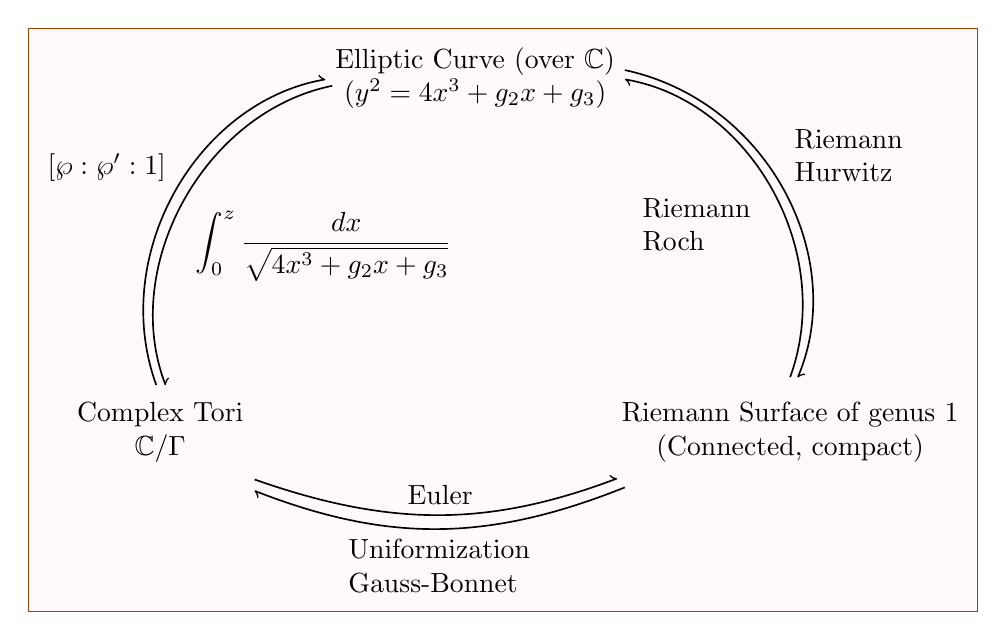
\begin{tikzpicture}[shorten >=3pt, >=left to,semithick]
\newlength\Ell \newlength\Com \newlength\Rie
\settowidth{\Ell}{\hspace{14pt}($y^2=4x^3+g_2x+g_3$)}
\settowidth{\Com}{\hspace{14pt}Complex Tori}
\settowidth{\Rie}{\hspace{14pt}(Connected,compact)}
\def\a{1.5} \def\b{4}
\path (0,2*\a) node[align=center](1){Elliptic Curve (over $\mathbb C$)\\ ($y^2=4x^3+g_2x+g_3$)};
\path (-\b,-\a) node[align=center](2){Complex Tori\\ $\mathbb C/\Gamma$};
\path (\b,-\a) node[align=center](3){Riemann Surface of genus $1$ \\ (Connected, compact)};

\draw[->] (-\Ell/2-1.2,2*\a-.1) 
to [xshift=3pt,bend right=50]node[below right]{$\displaystyle\int_0^z\frac{dx}{\sqrt{4x^3+g_2x+g_3}}$} (-\b,-\a+.5);
\draw[->] (-\b-0.05,-\a+0.6) 
to [bend left=50]node[above left](5){{$[\wp:\wp':1]$}} (-1.8,2*\a);
\draw[arrows={-left to}] (-\b+1.2,-\a-.6) 
to [bend right=20] node[above]{Euler} (\b-2.1,-\a-.55);
\draw[arrows={-left to}] (\b-2.1,-\a-.7) 
to [yshift=-3pt,bend left=20] node[below,xshift=1cm](4){\parbox{4.2cm}{Uniformization\\Gauss-Bonnet}} (-\b+1.1,-\a-0.6);

\draw[arrows={-left to}] (\b,-\a+.7) 
to [bend right=50] node[below left]{\parbox{1.5cm}{Riemann Roch}} (1.8,2*\a);
\draw[arrows={-left to}] (1.9,2*\a+.1) 
to [xshift=3pt,bend left=50]node[above right]{\parbox{2cm}{Riemann Hurwitz}} (\b-0.05,-\a+.6);
\begin{scope}[on background layer]
\node [draw=browne,fill=rede,fit=(1)(2)(3)(4)(5)] {};
\end{scope}



\end{tikzpicture}

\end{document}
